\documentclass{standalone}
\usepackage{tikz}
\begin{document}
    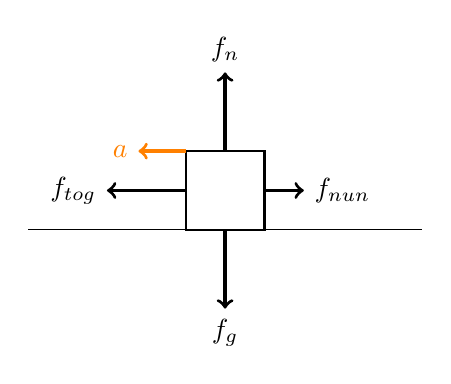
\begin{tikzpicture}
        % gólf
        \draw (0,0) -- (5,0);
        % kassi
        \draw [thick] (2,0) rectangle (3,1);
        % kraftar
        \draw [very thick, ->] (2.5,0) -- (2.5,-1) node [below] {$f_g$};
        \draw [very thick, ->] (2.5,1) -- (2.5,2) node [above] {$f_n$};
        \draw [very thick, ->] (2,0.5) -- (1,0.5) node [left] {$f_{tog}$};
        \draw [very thick, ->] (3,0.5) -- (3.5,0.5) node [right] {$f_{nun}$};
        % hröðun
        \draw [very thick, ->, orange] (2,1) -- (1.4,1) node [left] {$a$};
    \end{tikzpicture}
\end{document}
